% !TEX root = ../thesis-example.tex
%
\chapter{Introduction}
\label{sec:intro}

\cleanchapterquote{Astronomy? Impossible to understand and madness to investigate.}{Sophocles}{} \\

In this Part A Thesis I will summarize some of the work I have been doing the
first two years of my PhD, while also officially enrolled in the masters
programme. The work I have done is mainly divided into three subjects: Quasars,
GRBs and supernovae and is related to various aspects of the subjects. 

For QSOs, I have researched the average properties of a sample of bright $M_{r}
\leq -27.5$ QSOs and created a composite spectrum for community usage. I showed
an application of the composite in inferring dust content of the quasar host
galaxies. Additionally, I find a steeper slope of the quasar power-law continuum
as compared to the traditionally assumed one, indicating an intrinsically harder
continuum. This project therefore investigates both intrinsic properties of the
quasar phenomena, but also allows for the conditions of the intervening to be
inferred, both in the quasar host or potential absorption systems in the
line-of-sight.

For GRBs, I am involved with the X-shooter GRB collaboration and will be
investigating the average properties of the GRB optical afterglows for the
sample we are building. Data-collection for the sample is continuous and we have
an ESO TOO-program to do ground-based follow-up of the optical afterglow form
GRBs detected with \textit{Swift}.  I have developed an algorithm to normalize
the afterglows which is then used  as a product of the afterglow sample, for
example for the absorption-line studies. Once a sufficient sample size is
reached, I will lead a project to construct a composite afterglow spectrum. This
afterglow composite can then be used twofold: as a cross-correlation template to
determine redshift for future discovered noisy afterglows and as a way to
explore the average properties of the optical afterglows, thereby also allowing
identification of potentially interesting outliers for further observations. 

For SNe, I am involved in two projects. One related to the explosion
environments of type Ic and Ic-BL supernovae without accompanying GRBs, where we
have obtained a sample of 19 supernova host galaxies observed with an IFU,
allowing spatially resolved diagnostics to be calculated for the stellar
progenitor population, to investigate whether the explosion environments of the
two types of supernovae differ. This can be used to constrain the explosion
mechanisms for the different kinds of SNe. This project is in an indirect way
related to an investigation of the GRB progenitor system, because fast-ejecta
SNe are sometimes seen associated with GRBs and the reason why some GRBs have
SNe and others don't remains a mystery. The other supernova-project I am
involved with is a collaboration with the Frontier Fields program, where
spectroscopic follow-up of potential high-redshift supernovae are carried out
using X-shooter. The scientific rationale behind this project is the increased
chance of "serendipitously" discovering high-redshift SN in the Frontier Fields
because of the strong gravitational lensing the galaxy clusters targeted. If
high-redshift SN are of the Ia-type, this will help constrain our current
cosmology where the high-redshift SNe carry the highest leverage in terms of
discerning between different world-models. As part of this work I am working on
the quadruply lensed supernova "SN Refsdal" where the X-shooter observations
have helped constrain the SN type.

This report will present a brief status of the work that have been done in the
three fields and how it relate this to my own research. Apart from the research
I have been doing, I have taken 30 ECTS points distributed in the following
PhD-schools and regular courses: "Coping with the challengers of a PhD +
Scientific Writing", "Responsible Conduct of Research", "Introduction to
University Pedagogy", "Summer Schools in Statistics and Computation for
Astronomers", "Introduction to sub-mm interferometry and science with ALMA",
"Advanced Methods in statistical data analysis", "Classical Astrophysical
Papers". Additionally I have taught the 840 hours including Mechanics 1 and 2
courses for which I was awarded the Jens-Martin prize for excellence in
teaching.

I will conclude with an outlook of what I will be working on in the last two
years of my PhD. 
I attach the submitted quasar paper, and the advanced draft of the "SN Refdal"-paper with this Part A Thesis.

\clearpage

{\Large Publications} \\

{\large Paper I} \\
\textit{An X-shooter composite of bright $1<z<2$ quasars from UV to Infrared} \\
\textbf{Selsing, J}; Fynbo, J. P. U.; Christensen, L;  Krogager, J.-K. \\
\textit{Submitted to A\&A} \\

{\large Paper II} \\
\textit{Spectroscopic classification and confirmation of the first multiply imaged supernova}\\
P. L. Kelly, G. Brammer, \textbf{J. Selsing}, S. A. Rodney, J. Hjorth, R. J. Foley, L Christensen, and et al. \\
\textit{Advanced draft ready} \\


{\large Paper III} \\
\textit{Spectrophotometric analysis of GRB afterglow extinction curves with X-shooter} \\
J. Japelj, S. Covino, A. Gomboc, S. D. Vergani, P. Goldoni,\textbf{ J. Selsing}, Z. Cano, V. D'Elia, H. Flores, J. P. U. Fynbo, F. Hammer, J. Hjorth, P. Jakobsson, L. Kaper, D. Kopač, T. Krühler, A. Melandri, S. Piranomonte, R. Sánchez-Ramírez, G. Tagliaferri, N. R. Tanvir, A. de Ugarte Postigo, D. Watson, R. A. M. J. Wijers \\
\citet{Japelj2015} \\

{\large Paper IV} \\
\textit{GRB hosts through cosmic time - VLT/X-shooter emission-line spectroscopy of 96 GRB-selected galaxies at 0.1 < z < 3.6} \\
T. Krühler, D. Malesani, J. P. U. Fynbo, O. E. Hartoog, J. Hjorth, P. Jakobsson, D. A. Perley, A. Rossi, P. Schady, S. Schulze, N. R. Tanvir, S. D. Vergani, K. Wiersema, P. M. J. Afonso, J. Bolmer, Z. Cano, S. Covino, V. D'Elia, A. de Ugarte Postigo, R. Filgas, M. Friis, J. F. Graham, J. Greiner, P. Goldoni, A. Gomboc, F. Hammer, J. Japelj, D. A. Kann, L. Kaper, S. Klose, A. J. Levan, G. Leloudas, B. Milvang-Jensen, A. Nicuesa Guelbenzu, E. Palazzi, E. Pian, S. Piranomonte, R. Sanchez-Ramirez, S. Savaglio, \textbf{J. Selsing}, G. Tagliaferri, P. M. Vreeswijk, D. J. Watson, D. Xu \\
\citet{Kruhler2015} \\


\clearpage

\section{Quasars: Cosmic Lighthouses}
\label{sec:intro:qso}

The word quasar is derived from quasi-stellar radio source objects which is what
quasars were initially detected as: point-like radio sources without an optical
counterpart. When the first optical counterpart was discovered it indeed
resembled a blue star, but spectroscopic follow-up revealed a confusing pattern
with very broad emission lines superposed in a blue continuum. When the lines
were matched to the correct atomic species, a cosmological origin was
established which posed a problem for the mechanisms powering the source because
the extreme energies observed. The Eddington limit is the maximal luminosity a
gravitationally bound object of a given mass can have without radiation pressure
tearing the object apart and at the luminosities inferred from the cosmological
origin of the quasars and the observed brightness the required mass of the
source extremely high. One of the first quasars discovered, 3C 273, is estimated
to have a mass of $\sim900 \times 10^{6} M_\odot$ \citep{Peterson2004} which far
exceeds the maximal possible mass a star can have before it would immediately
collapse to a back hole \citep{Belczynski2010}. Quasars also exhibits a large
degree of variability in the observed flux on differing time-scales in the order
of weeks and years with shorter time-scale variability is superposed on longer
variability periods. The short time-scales observed requires a relatively small
emitting regions which poses a problem for a potential stellar origin of the
emission and gives merit to the idea of a black hole powering the emission.

The optical-to-ultraviolet emission mechanism of quasars are by now quite well
understood \citep{Elvis1994}. A supermassive black hole at the center of a
galaxy is surrounded by a hot accretion disc which emits a featureless thermal
continuum \citep{Shakura1973, Pereyra2006}. The central continuum photoionizes a
region of hot clouds, and further out, cold clouds which gives rise to lines
with both broad and narrow components \citep{Elvis2001}.  Varying conditions in
the clouds ensure that each ionic species have optimal conditions to produce
line emission \citep{Baldwin1995}. Despite the apparent different conditions in
which the emission arises, the overall shape of most quasar spectra look similar
\citep{Dietrich2002}. The remarkable uniformity of the average spectral
properties across luminosity and redshift indicate very similar underlying
physical mechanisms which can be understood in terms of Eigenvector 1
(\citep{Boroson1992, Francis1992}) where the Eddington ratio drives the relative
strength of the lines and orientation effects influences the observed kinematics
of the lines \citep{Shen2014a} accounting for the majority of the inter-quasar
variation. This means that the accretion rate and the mass of the black hole
largely determines the spectral appearance of a given quasar. Quasars are a part
of a more general class of objects called Active Galactic Nuclei (AGN) and the
different classes of AGN are in part believed to be viewing effects
\citep{Elvis2001}.


The average quasar spectrum of the sample presented in Paper I is shown in Fig.
\ref{fig:intro:qsospec} where the position of the most prominent emission lines
has been marked. The blue dashed line is a power-law fit to the spectral regions
deemed free of contaminating emission lines and it can be seen that a pure
power-law relatively well describes the continuum which is also the shape that
is predicted from \citep{Pereyra2006}.

\begin{figure}[htb]
	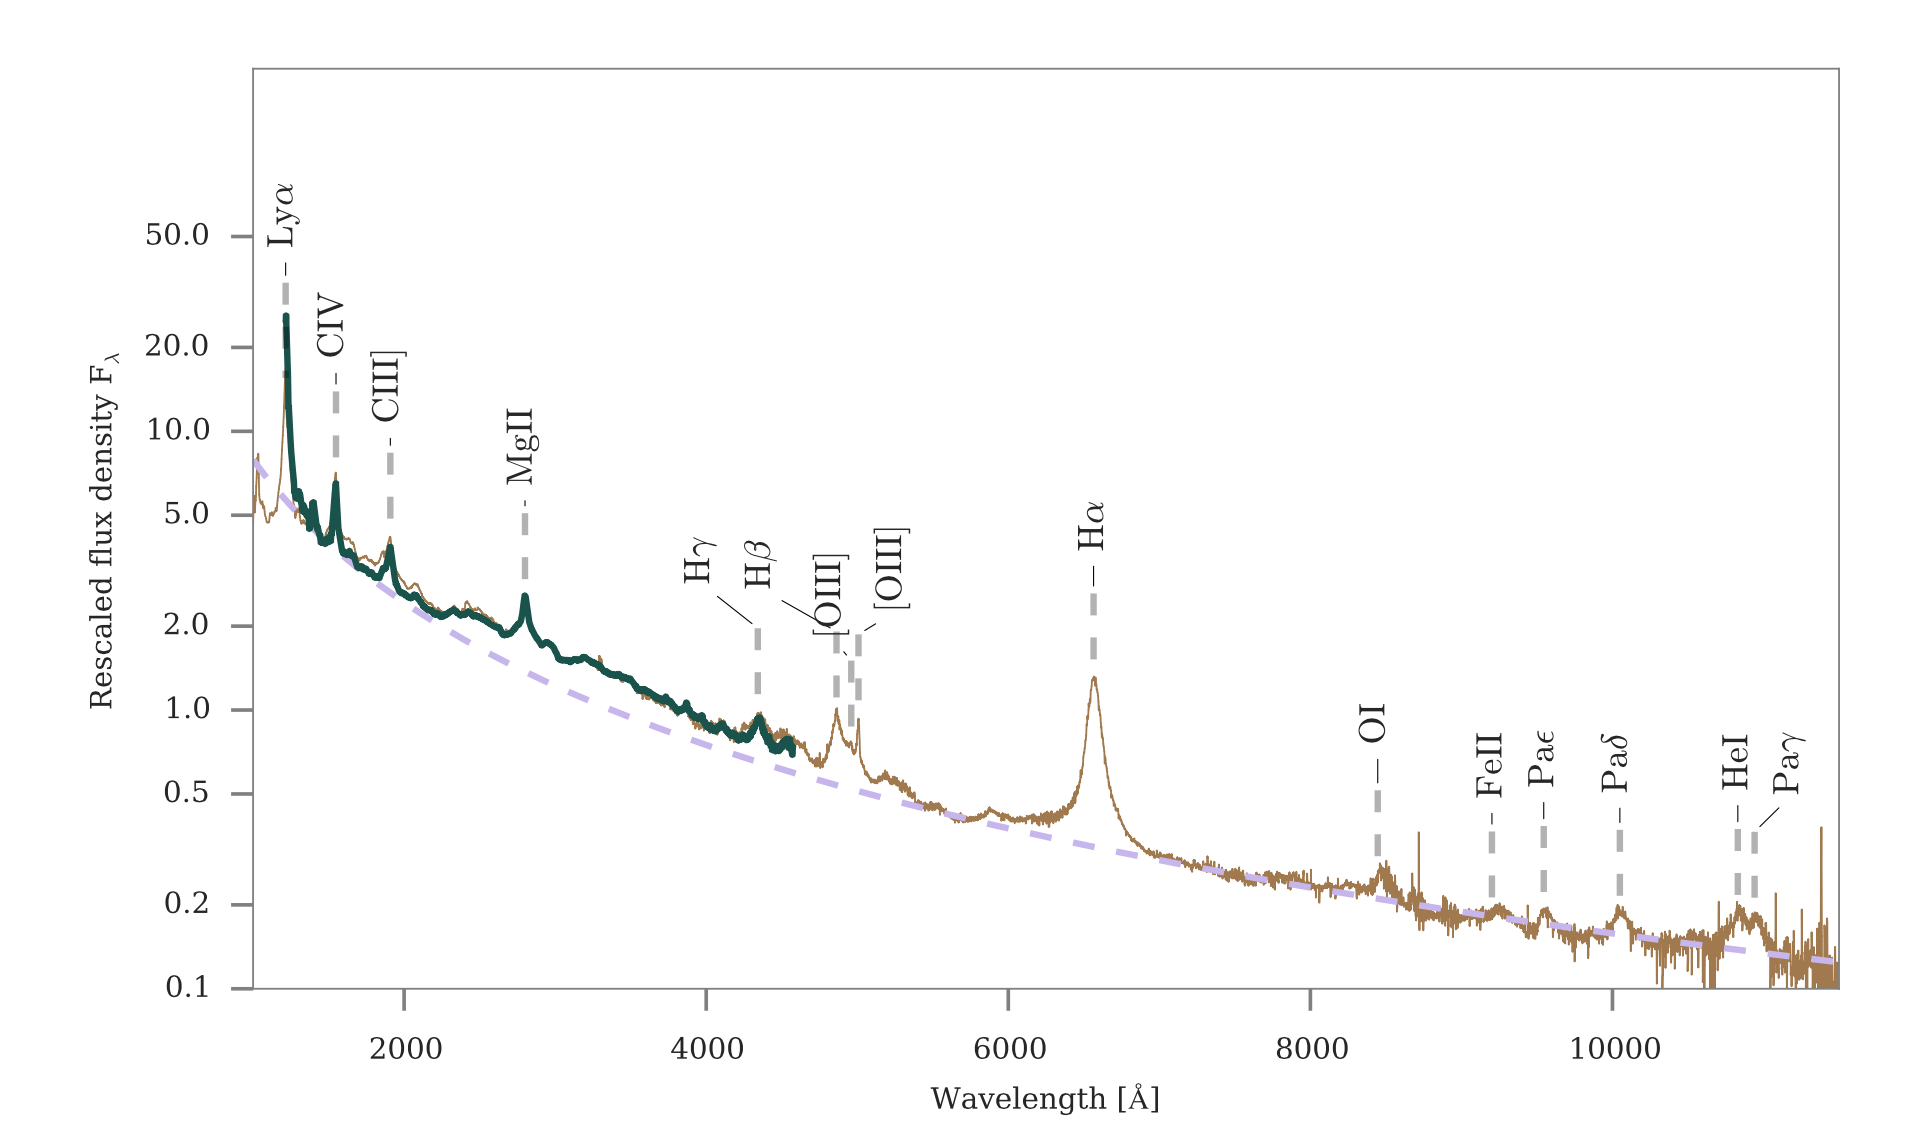
\includegraphics[width=\textwidth]{gfx/qsospec}
	\caption{Quasar composite spectrum from Paper I. The brown line is the average
quasar spectrum where several of the prominent lines have been marked. The blue
dashed line is a power-law fit to the regions free of contaminating emission and
 the dark green line is an average spectrum constructed for all SDSS spectra
fulfilling the selection criteria imposed on the sample observed with
X-shooter.}
	\label{fig:intro:qsospec}
\end{figure}


Even though the general principles behind the quasar phenomena seems to be
relatively well understood, important details remains especially in terms of
understanding the total contribution of the quasar feedback in regulating star
formation in galaxies \citep{DiMatteo2005}, how the first quasar became so
massive so rapidly after the creating of the universe \cite{Wu2015a}, how the
co-evolution of the quasars and their host galaxies works \citep{Ferrarese2000},
what role quasars played in reionization \citep{Hopkins2007} and what the full
sample of quasars look like \citep{Krawczyk2015}. The quasar contribution to
reionization depends on the quasar luminosity function (QLF) which in turn
depends on the assumed slope of the quasar SED. The QLF is the intregrated
luminosity of all quasars as a function of redshift and when calculating it, a
representative quasar SED model is required. The quasar optical SED is usually
is modelled by a power-law where the slope of the quasar continuum is determined
from the average slope og large samples of quasars \citep{Vandenberk2001,
Richards2006a, Shen2011, Lusso2015} where regions free of emission lines is
determined "by-hand". It is very efficient to build large samples of quasars
from SDSS \citep{Paris2014}, but the relatively modest wavelength coverage of
the instrument install at Apache Point Observatory \citep{Gunn2006} makes it
difficult to uniquely determine a representative slope. Work has been done to
extend the average quasar spectrum to higher wavelengths using other instruments
\citep{Glikman2006}, but a well defined sample of quasars with spectra covering
the entire range from ultra-violet to near-infrared has not been carried out.
The work I have carried out in Paper I seeks to address specifically this point
by observing 7 extremely bright, $M_{r} \leq -27.5$, quasars which will
therefore contain negligible amounts of host galaxy contamination. Additionally
the composite spectrum I have generated can be used to infer the dust content of
the quasar host galaxy and potential intervening absorption systems,
specifically Damped Lyman Alpha (DLA) systems. DLAs are defined as having
hydrogen column densities higher than $N_{\mathrm{HI}} > 2 \times 10^{20}
cm^{-2}$, determined from the equivalent width of the hydrogen absorption lines.
This class of objects are believed to be self-shielding systems of gas that
contain a significant fraction of the neutral hydrogen at redshift $z \sim 5$
\citep{StorrieLombardi2000}. Since these objects are only observed in
absorption, our understanding of these object depend heavily on our knowledge of
the illuminating object. An example of inferring the dust properties and amount
is \citet{Krogager2015}, where artificially reddening a composite quasar
spectrum is used to fit for the amount of dust under some assumed extinction
law. The quasar composite used in that work consists of the template by
\citet{Vandenberk2001} stitched together with the one by \citet{Glikman2006}, to
produce a quasar composite covering the range of wavelength investigated. Paper
I presents a single template that covers en entire region from a homogeneous
selection and hopefully it will see a great deal of community usage. The paper,
template and all the code used to generate the composite is made publicly
available at \url{https://github.com/jselsing/QuasarComposite} as a way to
encourage open source science.

\section{Gamma-Ray Bursts: Flashes in the Dark}
\label{sec:intro:grb}


The existence of GRBs was serendipitously discovered by the VELA satellites that
were launched to detect potential detonations of nuclear bombs in space and
could not have been discovered by earth-based telescopes due to the inability of
gamma-rays to penetrate earths atmosphere. Short flashes of gamma-rays were
detected for which a terrestrial origin could be excluded and a new celestial
phenomena had been discovered. 
Significant advances has been made, especially through the rapid, space-based
follow-up carried out with the BATSE \citep{Harmon2004} establishing the
cosmological origin of GRBs though the isotropic distribution of bursts
\citep{Meegan1992},  BeppoSAX \citep{Boella1997} which was the first instrument
to identify an X-ray counterpart  \citep{Costa1997} for which an optical
afterglow was found and later a host galaxy and the \textit{Swift}-satellite
\citep{Gehrels2004} finding afterglows for ground based follow-up, using all
available wavelengths. 

The GRB phenomena consists of mainly two observable phases. A prompt phase of
direct emission radiating up to a total of $10^{55} $ergs if the energy emitted
is isotropic, which is comparable to the entire universe \citep{Kumar2014} for
the duration of the burst and an afterglow phase which is believed to be
associated with the burst ejecta interacting with the circumburst material. The
prompt phase can last 1$^{-3}$ - 1$^3$ s with a clear bi-modality in the total
sample of burst durations pointing to two distinct populations of objects also
supported by the differing hardness ratio of the two types, with the short type
typically having a higher fluxes at shorter wavelengths. These two population
are classified af short GRBs if the duration is less than 2 seconds and long
GRBs if the duration is longer. 

The central engine for the bursts is still an open question, but the association
of long GRBs with supernova of type Ic-BL points to a massive stellar origin
\citep{Woosley2006, Hjorth2013}, where the association of a weaker "kilonova"
with the short GRBs is seen a sign for merger-driven explosion mechanism
\citep{Tanvir2013}. Several models exist to explain both types of burst, with
the collapsar-model being favored for the long GRB and neutonstar-neutronstar
merger favored for the short GRB. A common idea for both explosion mechanisms is
to explain the amount of energy released as accretion of matter onto a black
hole which as for the quasar emission mechanism can yield a very high yield in
terms of energy. For the long GRBs, the core of a massive, rapidly rotating star
collapses when the iron core exceeds the Chandrasekhar limit forming a black
hole. Through conservation of angular momentum an accretion disc is formed,
which via strong magnetic fields launches a jet that breaks out of the stellar
photosphere \citep{Woosley2006a}. The differing velocities of the ejected
material causes shocks inside the outflowing material which emit inverse
Compton-scattered synchrotron-radiation, bright in gamma-rays.  When the
swept-up material reaches the circum-burst material additional shocks are made
and the optical afterglow is created. A typical cartoon for this kind of
explosion mechanism is shown in Fig. \ref{fig:intro:grbglow}


\begin{figure}[htb]
	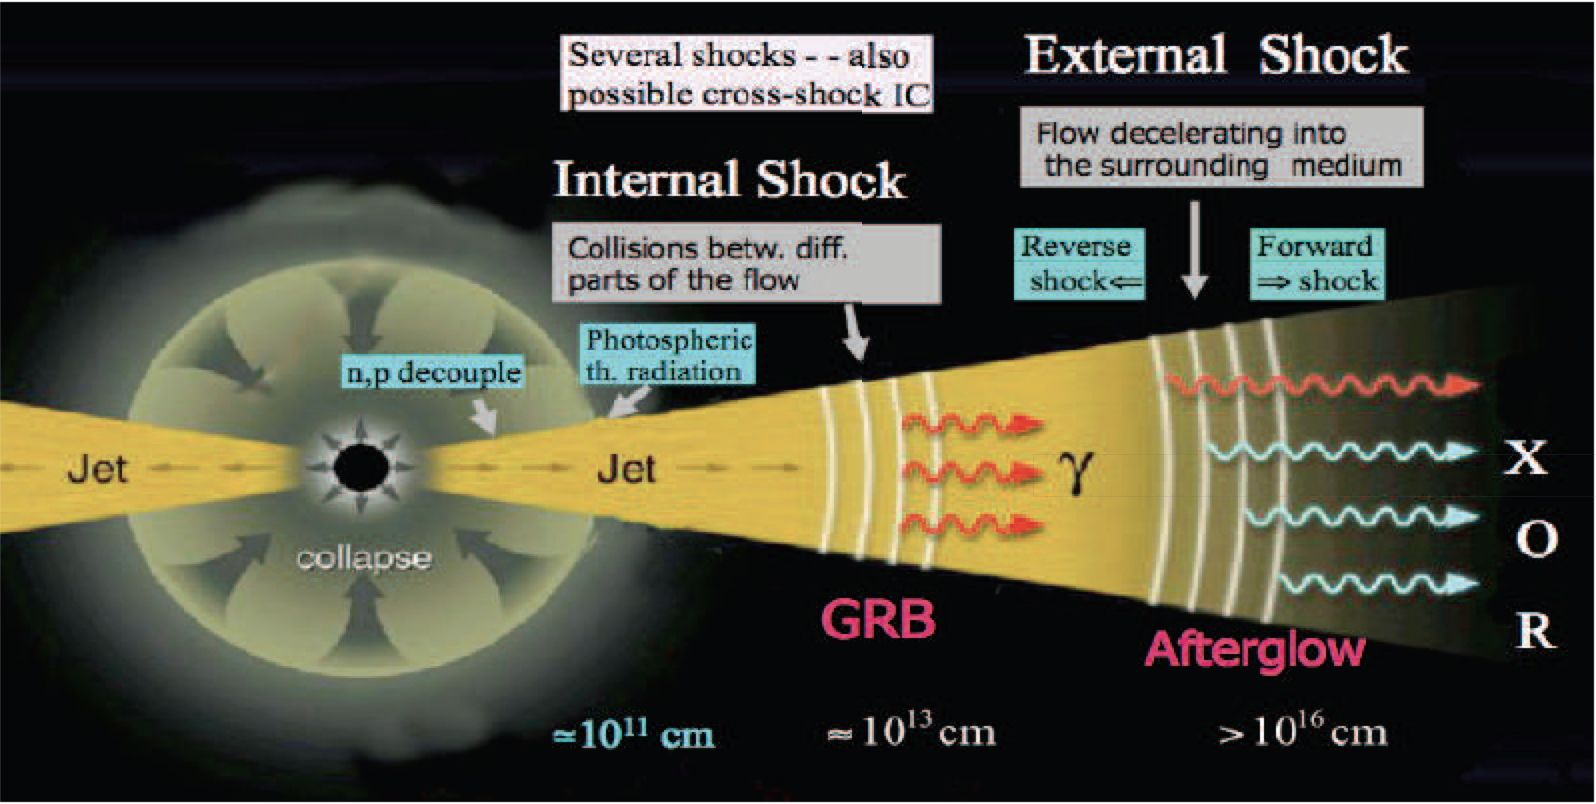
\includegraphics[width=\textwidth]{gfx/grbmec}
	\caption{Schematic view of the emission mechanisms in the traditional fireball
model. Schematic taken from \citet{Meszaros2014}}
	\label{fig:intro:grbglow}
\end{figure}

Because the explosion mechanism itself is hidden from sight inside the exploding
star, direct detection of the possible collapse is impossible. The prompt
emission is in many cases too short for detailed investigation so an informative
way to learn about the GRB explosion mechanism is to investigate the afterglow,
which is visible for longer periods of time, allowing for ground based
follow-up. Because the afterglow is a featureless continuum, just a with the
quasar, it can be used to infer the properties of the intervening material, both
in the host galaxy and in potential DLA systems. Since the sight-lines selected
by GRB afterglow are different than the ones selected by quasars, they provide
an independent view of the hosts of otherwise unobservable galaxies. Since the
quasars are always positioned in the , the center of the host galaxies and the
long GRBs are shown to trace the stellar light \citep{Fruchter2006,
Anderson2015}, this potentially could make a difference in the picture drawn.
Additionally, since GRBs are visible to such extreme redshifts
\citep{Salvaterra2009}, they provide a unique probe to select star formation at
the earliest times. 

A ground-based follow-up program has been undertaken using X-shooter, in which
all \textit{Swift}-bursts with galactic A$_{V} \leq 0.5$ and an XRT position
within 10 minutes are followed up, if possible. This program has led to a lot of
papers, investigating single bursts \citep[e.g.][to mention some]{Sparre2011,
DElia2014, Kruhler2013a, Xu2013a, DeUgartePostigo2014, Schulze2014a, Japelj2015,
Hartoog2015} which include GRBs with identified associated SNe, short GRBs and
detections of molecular hydrogen. 
In Paper III \citep{Japelj2015} we investigate the extinction shape in the host
galaxy at the position of the GRB for a sample of extincted afterglows. An
example of an extincted afterglow is shown in Fig. \ref{fig:intro:grbext} where
the spectrum is shown in black and the continuum level estimation shown in red.
From the normalized spectrum the neutral hydrogen column density can be
estimated and from the modeling the afterglow SED the preferred extinction law
can be inferred. For the sample of eight bursts we investigated here, there
seemed to be a preference for SMC-like dust towards the GRB sightlines. 
\begin{figure}[htb]
	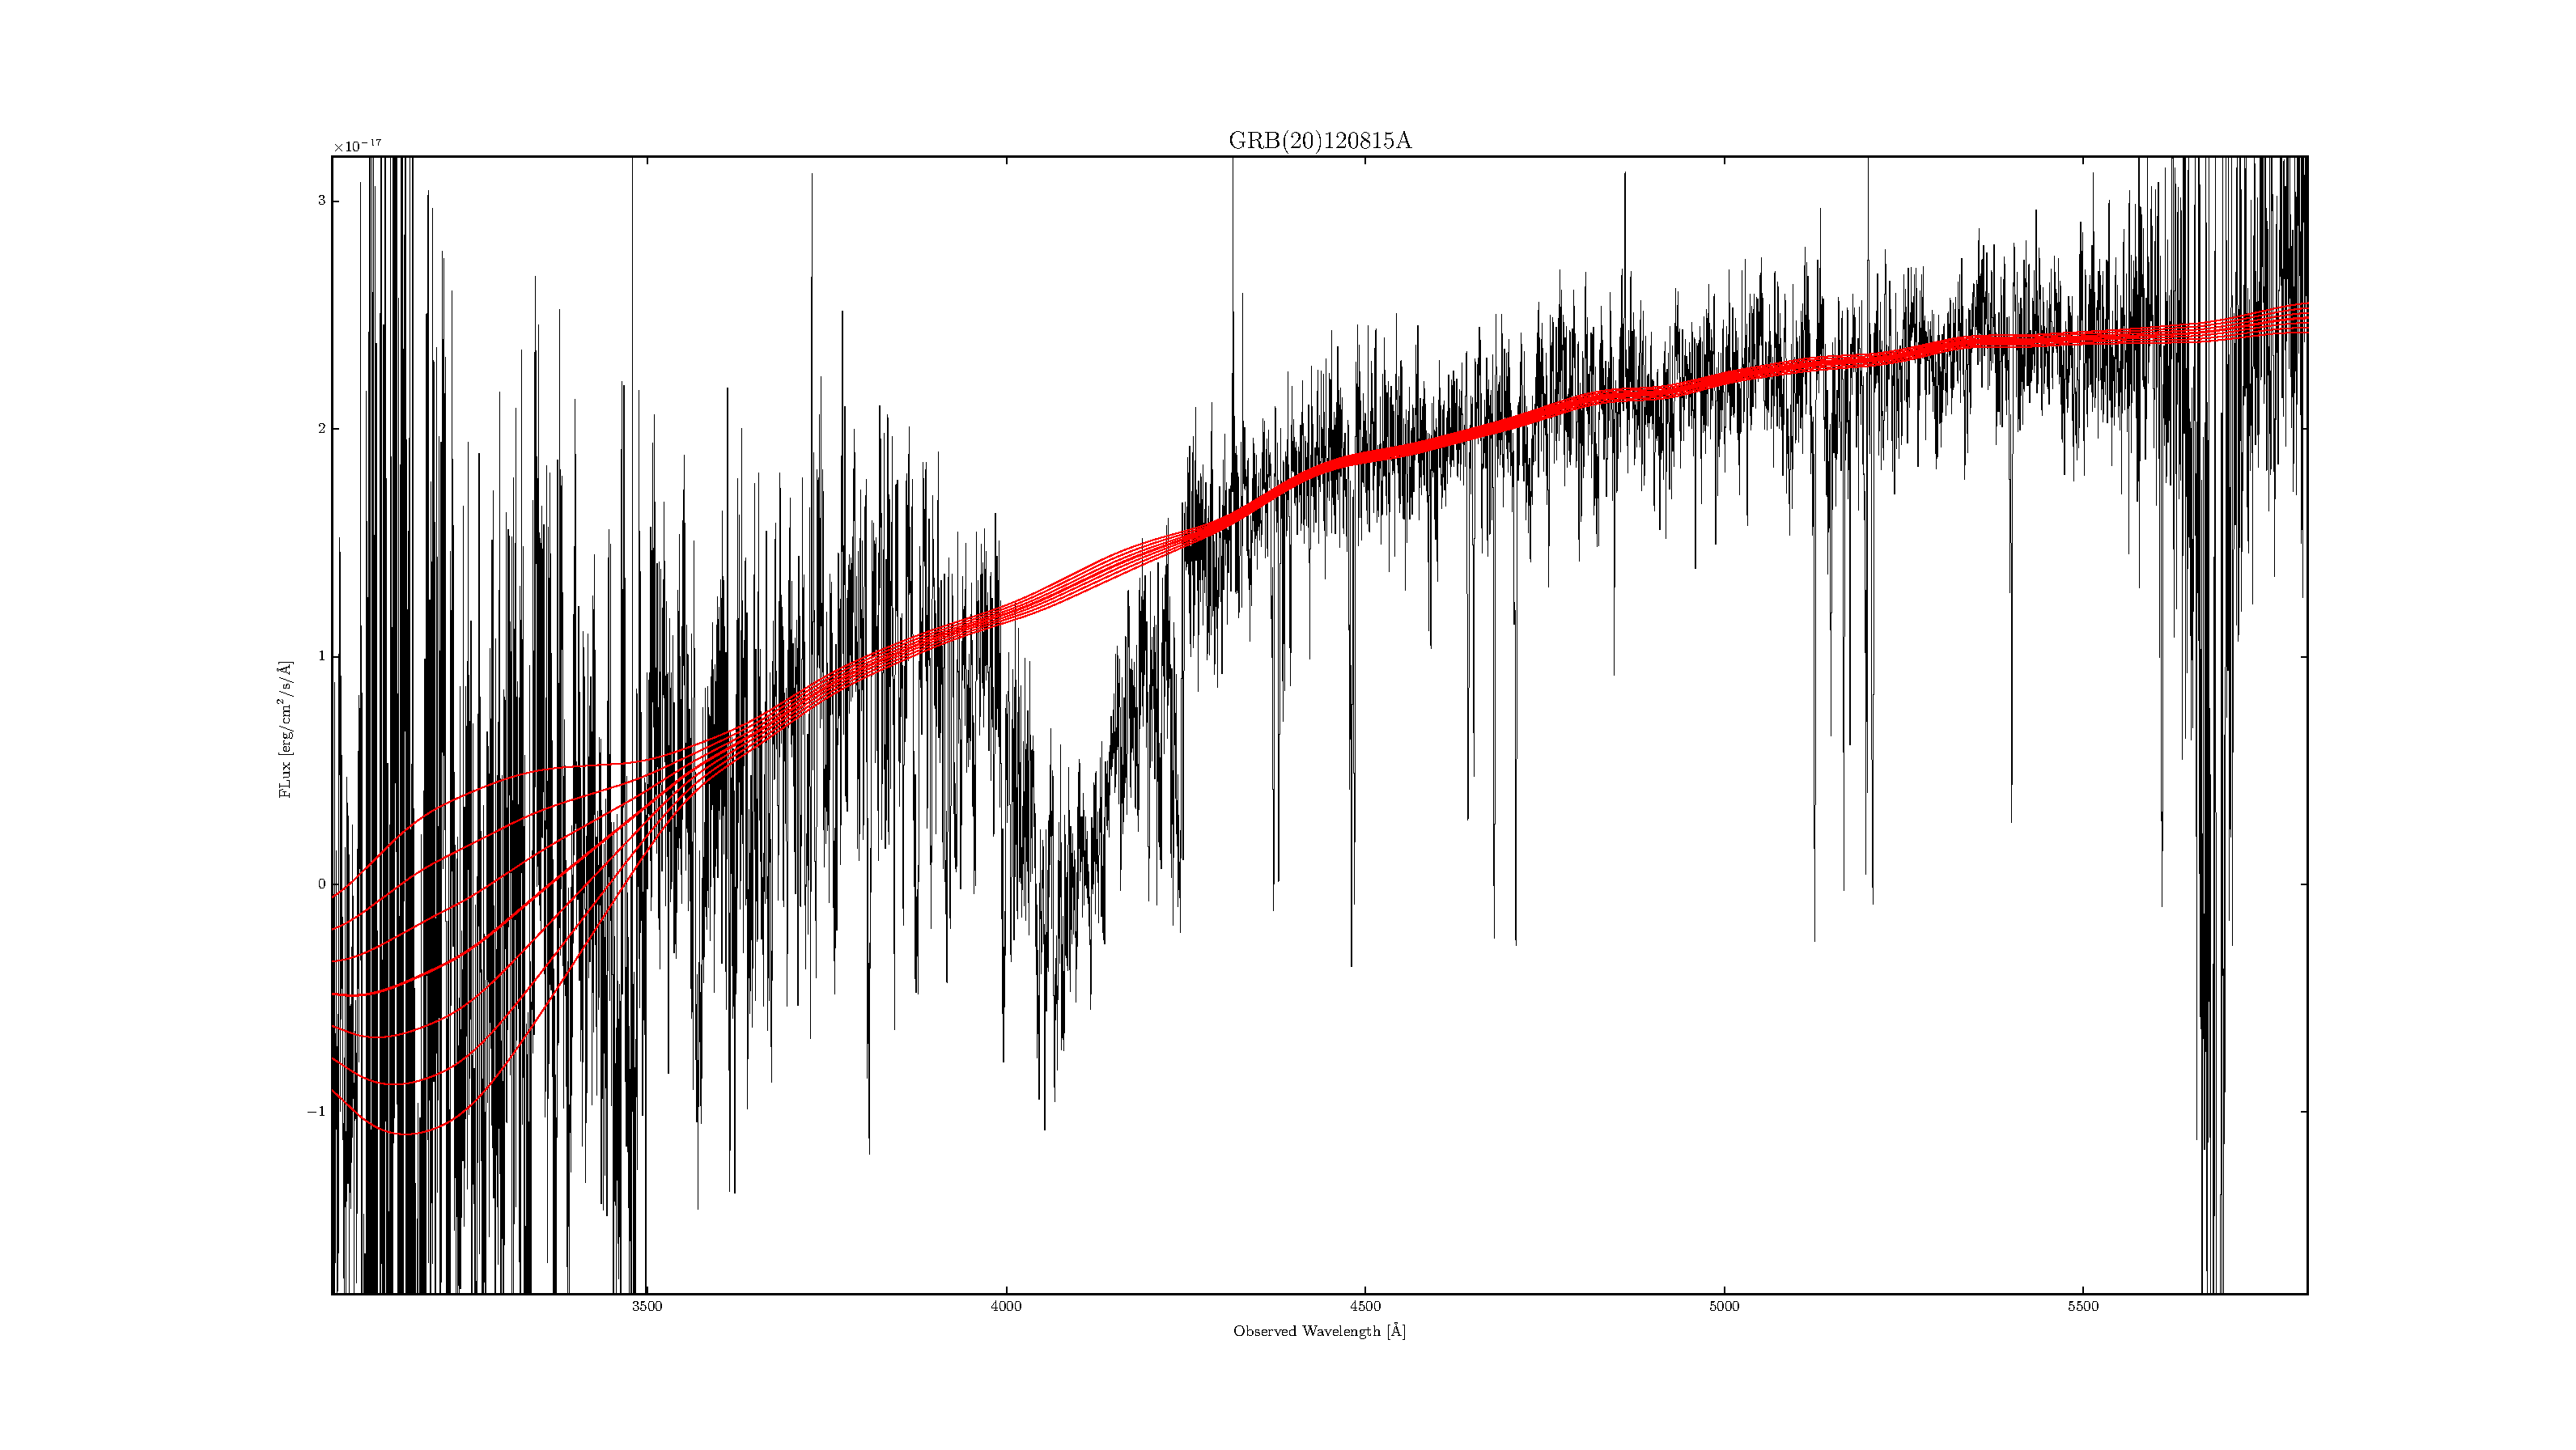
\includegraphics[width=\textwidth]{gfx/normspec}
	\caption{Extincted afterglow spectrum of GRB120815A in black. The broad
absorption feature at 4100 \AA~ is from Lyman $\alpha$ absorption in the host
indicating a redshift of $z \sim 2.35$. A multitude of narrow absorption lines
are visible in the spectrum belonging to various ionic species of elements. The
thick red line is the continuum level, as determined from the normalization
algorithm developed, the narrow red lines are the 1, 2, 3 $\sigma$ lines
indicating the uncertainty in the continuum placement. The continuum-level
algorithm will be presented in a future paper. }
	\label{fig:intro:grbext}
\end{figure}
Additionally, for some of the triggers that have been done only emission from
the GRB host galaxy if visible. The study of the host galaxies of GRBs is an
indirect way of investigating whether GRBs prefer unusual environments and if
the GRBs trace star formation. For a sample of 96 host galaxies, we have
investigated in paper IV \citep{Kruhler2015} whether there is a preference for
GRB to occur in metal-poor host as is expected from the theoretical explosion
models \citep{Woosley1993}, which would mean that GRBs cannot be used as a
representative proxy for star formation at high redshift and would have a bias
towards low -metallicity environments. What we showed in paper IV was that there
is indeed a preference for low metallicity host, but only at low redshift which
is attributed to the metallicity evolution of the universe where conversely at
redshift $z \sim 3$ most of the star formation in the universe takes place in
$Z_\odot \leq 0.5$ galaxies and thus the bias of GRB host towards lower
metallicities disappear.


\section{Supernovae: The fiery deaths of massive stars and their environments.}
\label{sec:intro:sn}

Some of nature's most powerful explosions, long
  GRBs and different kinds of core-collapse SN, are linked to the
  deaths of massive stars. However, neither the progenitor system nor
  the production conditions that lead to each kind of explosion in a
  massive stripped star are well understood. The different kinds of
  Supernovae (SNe) are determined by the initial mass and metallicity
  of the stellar progenitor, as well as by the metallicity-dependent
  mass loss in the stellar winds at the end phase of their evolution
  and the interaction with a sufficiently close companion star. Type
  Ic SNe (SNe Ic) are explosions from the most heavily stripped
  massive stars that have been removed of both their H and He
  layers. Long duration gamma-ray bursts (GRBs) may be the most
  extreme cases of stellar explosions, and a few cases have been
  associated with broad-lined Type Ic SN \citep{Woosley2006}, while other long GRBs
  surprisingly lacked the distinct SN signatures \citep{Fynbo2006}. The connection
  between long-duration GRBs and broad-lined SNe Ic (SNe
  Ic-bl/hypernovae) and the existence of SNe Ic-bl without observed
  GRBs raises the question of what distinguishes a GRB progenitor from
  that of an ordinary SN Ic-bl without a GRB. This question may be
  answered by observing the stellar progenitors, which give rise to
  the various types of SN explosions. However, searches for SN
  progenitors in images taken before the explosions have failed,
  because the galaxies are distant and individual stars are difficult
  to distinguish \citep{Maund2005}.

\hspace{0.4cm} An indirect method is to explore the environments at
the locations of the SN and GRBs to look for systematic trends. SN
Ic-bl without observed GRBs lie in systematically more metal rich
environments than SNe with GRBs \citep{Modjaz2008}. Integral field data of the host
of GRB\,980425/SN\,1998bw show that the location of the SN (a Type
Ic-bl) is close to a very metal poor region, but that the metallicity
variations in HII regions in the dwarf galaxy host are otherwise minor
\citep{Christensen2008}.  In comparison Fig. 1 shows the Type Ic sites to be relative
metal rich. Recently the abundances at the sites of different kinds of
core collapse SNe have been determined and shows that SNe Type Ic lie
in systematically more metal rich environments than other types of
core collapse explosions (Fig. 3) \citep{Modjaz2011, Leloudas2011, Kuncarayakti2013a, Kelly2012}.  In contrast \citet{Anderson2010} argue
that metallicity is not the dominant parameter for the SN type. The
metallicity difference may have a physical origin, as a higher
metallicity may give rise to stronger line-driven winds that remove
the outer H and He layers of the star \cite{Vink2005}, a necessary condition for
a Type Ic SNe. This argument does not explain the lower abundances at
the sites of SNe Ic-bl as well as at GRB regions, since GRB
progenitors are expected to be metal poor \citep{Woosley1993}, unless the GRB-SN
progenitors underwent a peculiar evolutionary phase marked by chemical
homogeneous mixing. %A possible solution to this dilemma is a massive
%binary progenitor system, rather than a metallicity effect.

\hspace{0.4cm}
Using integrated central oxygen abundance of the host
galaxy as a proxy for the SN site \citep{Prieto2008, Kelly2012}, adopting the
luminosity-metallicity relation for SDSS galaxies \citep{Tremonti2004}, gives
systematically larger abundances than those measured in the SNe regions \citep{Modjaz2011}.
This offset is not surprising since galaxies targeted for SNe searches
are more luminous and massive and consequently have higher abundances
and they can have abundance gradients in their disks.
% Modjaz et al. include SNe found in both targeted surveys and
% serendipitously detected SNe.  although including both targeted and non
%targeted galaxies should mitigate systematic effects.
To understand SN progenitors it is important to establish the
systematic effects, which arise from the oxygen abundance
determinations, when only an integrated spectrum can be obtained
(e.g. low-luminosity or distant, unresolved galaxies), as well as the
implications of metallicity gradients in large massive galaxies.









Over the past decade, the deep HST Treasury surveys (GOODS, CANDELS, CLASH) have
all enabled "piggy- back" Type Ia SN searches, which have collectively
accumulated scores of SN detections that reach to uniquely high redshifts
\citep{Riess2007, Rodney2014b, Graur2014}.  
The ongoing HFF program now provides a powerful new tool for the discovery of
particularly high-z SNe. What sets this survey apart is the unique depth of each
visit, reaching m$_{lim,3\sigma}$(F160W) $\sim$27.9 (AB), $\sim$ 1 mag deeper
than CANDELS/CLASH per epoch. Gravitational lensing in the prime fields can also
magnify fluxes significantly, making it possible to detect distant background
events. 
The Hubble Frontier Field survey thus provides the first opportunity to discover
SNe at 2 < z < 3, building up a small but important “New Frontier” sample.
Because Type Ia SNe are standardizable candles, we can used lensed SNe Ia to
directly measure the true lensing magnification $\mu$ and confront the
predictions from existing lens models \citep[e.g.][]{Riehm2011, Li2012,
Patel2014}. Figure 1 shows a Type Ia SN with a magnification $\mu$ = 2.00 $\pm$
0.19 found in our HFF SN programme \citep{Rodney2015}. The magnification of this
SN is systematically overestimated by all existing mass models, with some
discrepant by > 5$\sigma$. Thus, our sample of lensed SNe Ia is already proving
to be a very valuable tool for testing galaxy cluster dark matter models, which
will be particularly valuable for the study of z > 8 galaxies magnified by these
clusters \citep[e.g.][]{Zheng2012}.
The unique combination of deep imaging, strong lensing, and rapid cadence in the
HFF program has also pro- vided two very exciting discoveries of multiply-imaged
transients. In January and August of 2014, we observed two short transient
events in separate images of the same strongly lensed galaxy, measured to be at
z=1.005 with X-shooter (Figures 1 and 2). Collectively nicknamed “Spock”, both
of these events are too faint to be a normal SN and too bright to be a stellar
flare. The light curves are also faster than expected from a He shell explosion
on a white dwarf \citep[a “.Ia” event][]{Bildsten2007}, and fainter than any of
the “fast optical transients” yet seen in wide-field ground-based surveys
\citep[e.g.][]{Kasliwal2010, Poznanski2010a, Vinko2014}.
Lens models (and Occam’s razor) suggest that these two events are most likely
spatially coincident on the source plane. If the two events were also coincident
in time, then this could be an example of an extremely rare neutron star
collision \citep[a “kilonova”][]{Tanvir2013, Barnes2013}. If not, these may be
two separate outbursts from an extremely bright nova with a remarkably fast
recurrence timescale of $\sim$1 year. This would be a unique nova, as it would
have a recurrence timescale on par with the most extreme examples known
\citep{Tang2014} and would also be at least an order of magnitude more luminous
than a typical nova.
In November of 2014 we discovered another exciting transient, this time with
four distinct sources appearing almost simultaneously in a strongly lensed
spiral galaxy at z = 1.5. Dubbed “SN Refsdal,” this is the first ever example of
a strongly lensed SN with multiple resolved images \citep[][Figure
3]{Kelly2014}. The Einstein Cross configuration is generated by a galaxy-scale
lens, but the SN host galaxy is also multiply imaged by the cluster, so we
expect to see SN Refsdal return elsewhere in the cluster field in 1–5 years
\citep{Oguri2015, Sharon2015}. Measurements of the relative magnifications and
time delays among these multiple images will soon deliver an unprecedented suite
of powerful new mass model constraints.



